


\documentclass[aspectratio=169]{beamer}
\usepackage[english]{babel}
\usepackage[latin1]{inputenc}
\usepackage{times}
\usepackage[T1]{fontenc}
\usepackage{hyperref}
\usepackage{graphicx}
\usepackage{xcolor}
\usepackage{verbatim}
\usepackage{listings}
\usepackage{textcomp}
\usepackage[framed,autolinebreaks,useliterate]{mcode}
\setbeamercovered{transparent=25}
%\usetheme{Darmstadt}
\usetheme{default}
\usecolortheme{default}
\setbeamertemplate{itemize items}[default]
\setbeamertemplate{enumerate items}[default]


\definecolor{mygreen}{rgb}{0,0.6,0}
\definecolor{mygray}{rgb}{0.5,0.5,0.5}
\definecolor{mymauve}{rgb}{0.58,0,0.82}

\lstdefinelanguage{Julia}%
{morekeywords={abstract,break,case,catch,const,continue,do,else,elseif,%
		end,export,false,for,function,immutable,import,importall,if,in,%
		macro,module,otherwise,quote,return,switch,true,try,type,typealias,%
		using,while},%
	sensitive=true,%
	morecomment=[l]\#,%
	morecomment=[n]{\#=}{=\#},%
	morestring=[s]{"}{"},%
	morestring=[m]{'}{'},%
}[keywords,comments,strings]

\lstset{ %
	language=Julia,                % choose the language of the code
	basicstyle=\footnotesize,       % the size of the fonts that are used for the code
	numbers=left,                   % where to put the line-numbers
	numberstyle=\tiny\color{mygray},  % the style that is used for the line-numbers
	stepnumber=1,                   % the step between two line-numbers. If it is 1, each line will be numbered
	numbersep=5pt,                  % how far the line-numbers are from the code
	backgroundcolor=\color{white},  % choose the background color. You must add \usepackage{color}
	showspaces=false,               % show spaces adding particular underscores
	showstringspaces=false,         % underline spaces within strings
	showtabs=false,                 % show tabs within strings adding particular underscores
	frame=single,                   % adds a frame around the code
	rulecolor=\color{black},        % if not set, the frame-color may be changed on line-breaks within not-black text (e.g. comments (green here))
	tabsize=2,                      % sets default tabsize to 2 spaces
	captionpos=b,                   % sets the caption-position to bottom
	breaklines=true,                % sets automatic line breaking
	breakatwhitespace=true,         % sets if automatic breaks should only happen at whitespace
	title=\lstname,                 % show the filename of files included with \lstinputlisting;
	keywordstyle=\color{blue},      % keyword style
	commentstyle=\color{mygreen},   % comment style
	stringstyle=\color{mymauve},    % string literal style
}



\AtBeginSection[]
{
  \begin{frame}<beamer>
    \frametitle{Outline}
    \tableofcontents[currentsection]
  \end{frame}
}

% script in Julia
% Julia project
% setting up Julia

\title{Introduction to Economic Modelling in Julia}
\subtitle{IFS TECH}
\author{David Sturrock}
\date{12th July 2023}


\begin{document}

\begin{frame}
  \titlepage
\end{frame}


\begin{frame}{Julia}

Julia is:
\begin{itemize}
	\item \dots a programming language
	\item \dots increasingly used across the natural sciences and economics
	\item \dots open source and with a growing community
\end{itemize}
\pause

\vspace{0.5cm}
Julia is useful to applied economists for:
\begin{itemize}
	\item \dots things requiring a lot of computation/optimisation
	\item \dots like estimating models through indirect inference (i.e. simulated method of moments)
\end{itemize}
\pause

\vspace{0.5cm}
Julia is not so useful for:
\begin{itemize}
	\item \dots `standard' data analysis
	\item \dots things using advanced/particular econometrics
\end{itemize}


\end{frame}


\begin{frame}{Installation and Setup}

\begin{itemize}
\item \textbf{Downloading and installing Julia:} Download the Julia language from \url{https://julialang.org/downloads/} and install.

\vspace{0.5cm}
\item \textbf{Setting up Julia in Visual Studio Code:}

    \begin{enumerate}
        \item Download and install Visual Studio Code if not yet installed: \url{https://code.visualstudio.com/download}.
        
        \item Launch VS Code, go to the Extensions view by clicking on the Extensions icon in the Activity Bar on the side of the window

        \item In the Extensions view, search for `Julia` and install the extension named `Julia`. Make sure this extension is enabled.

        \item Configure the Julia extension to use the Julia executable that you installed. To do this, open the command palette (`Ctrl+Shift+P`), type in `Preferences: Open User Settings`, and hit enter. In the settings tab, search for `Julia: Executable Path` and fill in the path to the Julia.exe file.

    \end{enumerate}
\end{itemize}

\end{frame}


\begin{frame}{What is special about Julia?}


\vspace{0.5cm}
\begin{enumerate}
	\item Both very fast and easy to use
	\begin{itemize}
		\item Julia combines interpretation and `Just-in-Time compilation' 
		\item Ease of interpreted languages (Matlab) while nearly as fast as C/Fortran
		\begin{itemize}
			\item e.g. can run interactively and debug easily
		\end{itemize}
	\end{itemize}

	\vspace{0.5cm}
	\item `Multiple dispatch'
	\begin{itemize}
	\item Functions can be defined generically and specialised by use
	\item Makes code more versatile while facilitating speed
	\end{itemize}	
	
	\vspace{0.5cm}
	\item Built-in parallel and distributed computing capabilities

	\vspace{0.5cm}
	\item `Expressive syntax'
	\begin{itemize}
		\item Code can be made to resemble mathematical notation
	\end{itemize}

	\vspace{0.5cm}
	\item Open source
	\begin{itemize}
	\item It's free! And consequently has a growing groups of users
\end{itemize}	
\end{enumerate}

\vspace{1cm}



% Note: compiled languages take the code you write, turn it into an optimised machine readable version and then run this.
% interpreted languages are run line-by-line (like stata code or matlab).
% compiled languages need you to declare types of variables and function inputs and harder to debug
% Julia combines both by e.g. allowing specialisation of functions based on arguments
% can also run parts of code interactively like an interpreted language
\end{frame}

\begin{frame}{Comparing Julia to other languages}

There are a range of languages that can be used for economic modelling
\begin{itemize}
	\item Matlab, Fortran, C++, C, Python, R(?)...
\end{itemize}
\vspace{0.5cm}

  \begin{tabular}{|c|c|c|c|c|}
	\hline
	\textbf{Item} & \textbf{Costly/Free?} & \textbf{Slow/Fast?} & \textbf{Hard/Easy-to-use?}  & \textbf{Less/more support}  \\
	& & & & \textbf{and packages?} \\
	\hline
	Fortran & \checkmark & \checkmark \checkmark & $\times$ & \checkmark \checkmark  \\
	\hline
	C/C++ & \checkmark & \checkmark \checkmark & $\times$ & \checkmark \checkmark \\
	\hline
	Julia & \checkmark & \checkmark & \checkmark & \checkmark  \\
	\hline
	Matlab & $\times$ & $\times$ & \checkmark \checkmark & \checkmark \\
	\hline
	Python & \checkmark & $\times$ & \checkmark & \checkmark \\
	\hline
	R & \checkmark & $\times$ $\times$  & \checkmark & \checkmark \checkmark \\
	\hline
\end{tabular}

\vspace{0.5cm}
\begin{itemize}
	\item All of this depends on your previous programming, what you are doing, and subjective judgement
\end{itemize}

\end{frame}

\begin{frame}{Basic Syntax of Julia}

\textbf{Variables}: defined without needing a specific type, e.g.
    \begin{itemize}
        \item \texttt{x = 5} (Integer)
        \item \texttt{y = 3.14} (Float)
        \item \texttt{str = "Hello"} (String)
    \end{itemize}

\vspace{0.25cm}

\textbf{Arrays}: Created using square brackets, indexed from 1.
\begin{itemize}
	\item e.g., \texttt{A = [1, 2, 3]} (column vector) ; \texttt{B = [1 2 3]} (row vector)
	\item \texttt{A[1]} would give `1'.
\end{itemize}
   
\vspace{0.25cm}

\textbf{Mathematical operations}: standard operators are used:  \texttt{+}, \texttt{-}, \texttt{*}, \texttt{/} etc.
\begin{itemize}
	\item put a `\texttt{.}' first to do element-wise on arrays
	\item i.e. \texttt{B*A} would give 14. \texttt{A.*A} would give \texttt{[1, 4, 9]}
\end{itemize}

\vspace{0.25cm}

    
\textbf{Comments}: use `\#'; multi-line comments between `\texttt{\#=}' and `\texttt{=\#}'
    

\end{frame}

\begin{frame}[fragile]{Functions}

We can create a simple function with the following text:
\vspace{-0.5cm}
\begin{lstlisting}
function square_then_double( input )
# This function outputs the twice the square of the input

output = 2 * (input.^2)

return output
end
\end{lstlisting}
\vspace{-0.5cm}
Rather than having in the main script, we save it as e.g. \mcode{square_then_double.jl}.

\vspace{0.5cm}

To use this function, we need to `include' the file that defines it in our main script:
\vspace{-0.5cm}
\begin{lstlisting}
include("functions/square_then_double.jl")
E = square_then_double(A)
\end{lstlisting}
\vspace{-0.5cm}
This code assigns the value \texttt{[1, 4, 9]} to \mcode{E}.

\end{frame}

\begin{frame}{Other things to note}

\textbf{Scope}
\begin{enumerate}
	\item Variables are defined globally by default
	\item Functions return only the final output by default; specify more with `return'
	\item Functions will only \textit{modify} inputs if return and re-assign
\end{enumerate}

\vspace{0.5cm} 

\textbf{Packages}
\begin{enumerate}
	\item To use additional packages, write \mcode{using `packageName'} at start of script
	\begin{itemize}
		\item useful packages include Distributed, Interpolations, QuadGK, Optim, Roots, LinearAlgebra, Random, Plots, Queryverse, XLSX, Statistics
	\end{itemize}
	\item To use parrallelisation, use the (built-in) ``Threads'' package
\end{enumerate}

\end{frame}

\begin{frame}{Example usage: estimating a lifecycle model of saving}

\textbf{Question}
\begin{enumerate}
	\item Are younger generations are less `patient' than older generations?
\end{enumerate}

\vspace{0.5cm} 

\textbf{Method}
\begin{enumerate}
	\item Build model of optimal wealth accumulation given economic conditions
	\item Estimate preference parameters by matching model to wealth data with simulated method of moments
\end{enumerate}

\vspace{0.5cm} 

\textbf{Why a quantitative model?}
\begin{enumerate}
	\item There is no closed-form solution for optimal saving in the face of uncertain future earnings, rates of return, changing household composition etc.
	\item Need to solve for optimal choices using numerical methods, which involves solving hundreds of optimisation problems
\end{enumerate}

\end{frame}

\begin{frame}{Example usage: estimating a lifecycle model of saving}

\begin{figure}
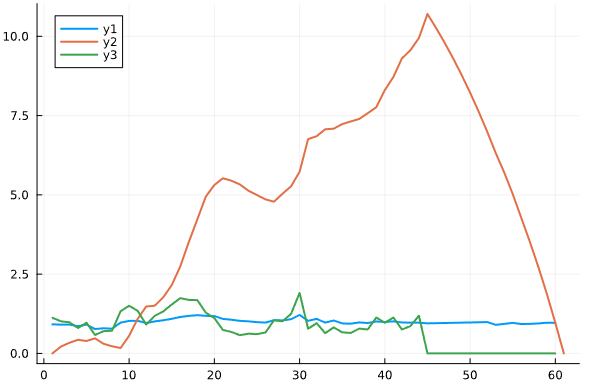
\includegraphics[height=0.7\textheight]{figures/lifecycle1.png}
\end{figure}

\end{frame}



\begin{frame}{Example usage: estimating a lifecycle model of saving}

\begin{figure}
	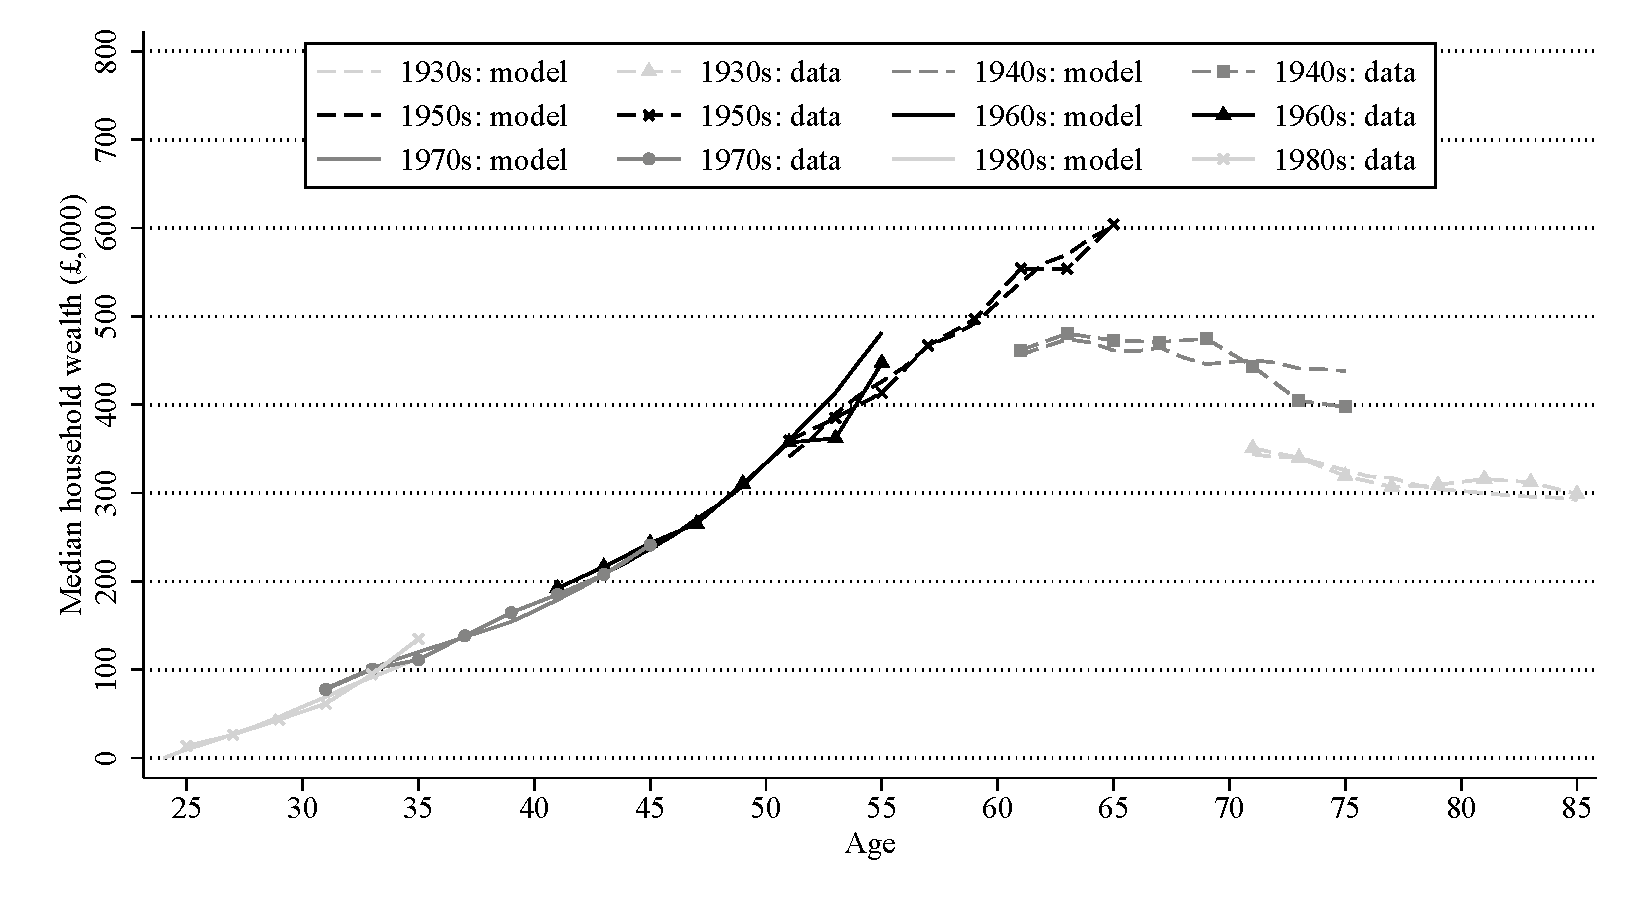
\includegraphics[height=0.8\textheight]{figures/Model_fit_all_gens.pdf}
\end{figure}

\end{frame}


\begin{frame}{Final thoughts}
\begin{itemize}
\item When solving things numerically, you never know what the correct answer is
\item Can never absolutely verify that there is no mistake
\item Calls for disciplined coding practices:
\begin{itemize}
\item Write many many many checks and warnings into your code
\item Once you think your program works - try to break it by stress-testing - select extreme parameters - may help you find bugs
\end{itemize}
\end{itemize}

\vspace{0.5cm}
Other good resources:
\begin{itemize}
	\item \url{https://github.com/cpfiffer/julia-bootcamp-2022}
\end{itemize}

\end{frame}


\end{document}



